\section*{Appendix A - General} \label{append:a}
Link to the Ethics form and Participant Information Sheet:

\url{https://falmouthac-my.sharepoint.com/:f:/g/personal/to231922_falmouth_ac_uk/EiE3vOcxqLlLuU0_BN7m1NoBCja231kbqKHAxOlqX-sRfw?e=4dc65R}
\\
\\
Link to the Computing Artefact GitHub repository: 
\url{https://github.falmouth.ac.uk/TO231922/computing-artefact}
\begin{figure}[ht]
    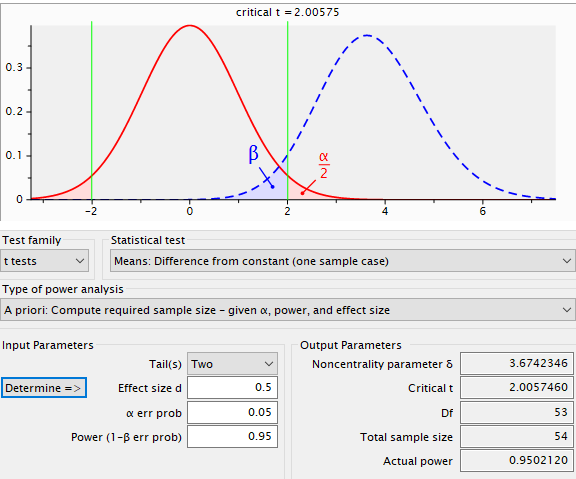
\includegraphics[width=\columnwidth]{./Images/gpower.png}
    \centering
    \caption{G*Power Sample Size}
    \label{gpower}
\end{figure}

\section*{Appendix B - Reflective Addendum} \label{append:b}


\newpage
\section*{Appendix C - Software Architecture} \label{append:c}
\begin{figure}[!h]
    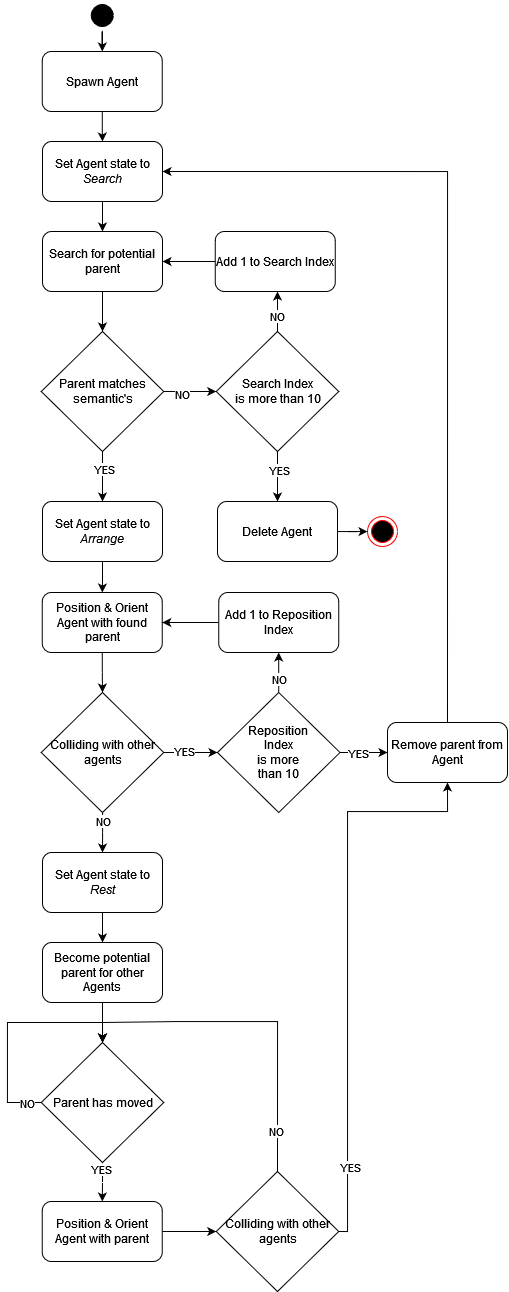
\includegraphics[width=\columnwidth]{./Images/AgentActivityDiagram.png}
    \centering
    \caption{Agent Behaviour represented in an Activity Diagram}
    \label{activity-diagram}
\end{figure}

\newpage
\section*{Appendix D - Testing} \label{append:d}
The Unit tests for my artefact were created using Unity's Test Framework and were used throughout the Artefact's development to validate the code and to ensure the Artefact worked as intended. Unit testing code can be seen in \hyperref[append:f]{Appendix F} and passed Unit Tests can be seen in Fig~\ref{unit-tests}.
\\
A small pilot study was conducted with the help of some BSc peers. This pilot study was conducted to ensure the validity of my experimental design. It consisted of them taking part in my 2-staged A/B test, helping in testing the effectiveness of how information was being represented - any feedback received from this small study was implemented into my methodology and no data from this pilot study was used within my data analysis.

\begin{figure}[ht]
    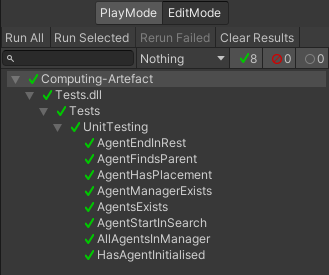
\includegraphics[width=\columnwidth]{./Images/unit-tests.png}
    \centering
    \caption{Unit Tests in the Unity Test Runner}
    \label{unit-tests}
\end{figure}

\newpage
\newpage
\section*{Appendix E - R Code} \label{append:e}
\lstinputlisting[language=r, label=StageOneRCode,caption=R Code for Stage One data., captionpos=b]{Code/StageOneRCode.R}

\lstinputlisting[language=r, label=StageTwoRCode,caption=R Code for Stage Two data., captionpos=b]{Code/StageTwoRCode.R}

\newpage
\section*{Appendix F - Unit Testing Code} \label{append:f}
\lstinputlisting[language=csh, label=UnitTestCode, caption=Unit Test Code used to validate the Artefact's code., captionpos =b]{Code/UnitTesting.cs}